\documentclass[11pt,a4paper]{article}

% Packages
\usepackage[utf8]{inputenc}
\usepackage[T1]{fontenc}
\usepackage{geometry}
\usepackage{amsmath,amssymb}
\usepackage{graphicx}
\usepackage{xcolor}
\usepackage{enumitem}
\usepackage{tcolorbox}
\usepackage{tikz}
\usepackage[hidelinks]{hyperref}
\usepackage{fancyhdr}
\usepackage{titlesec}
\usepackage{booktabs}
\usepackage{array}
\usepackage{listings}
\usepackage{multicol}
\usepackage{mdframed}

% TikZ libraries
\usetikzlibrary{shapes,arrows,positioning,fit,calc}

% Page geometry
\geometry{margin=0.9in}
\setlength{\headheight}{14pt}

% Colors
\definecolor{pytorchcolor}{RGB}{238,76,44}
\definecolor{conceptbg}{RGB}{240,248,255}
\definecolor{codebg}{RGB}{248,248,248}
\definecolor{importantbg}{RGB}{255,250,230}
\definecolor{tipbg}{RGB}{240,255,240}
\definecolor{warningbg}{RGB}{255,245,245}
\definecolor{codegreen}{RGB}{0,128,0}
\definecolor{codegray}{RGB}{128,128,128}
\definecolor{formulabg}{RGB}{245,245,255}

% Code listing style
\lstset{
    language=Python,
    basicstyle=\ttfamily\small,
    keywordstyle=\color{pytorchcolor}\bfseries,
    commentstyle=\color{codegray}\itshape,
    stringstyle=\color{codegreen},
    breaklines=true,
    frame=single,
    backgroundcolor=\color{codebg},
    showstringspaces=false,
    tabsize=4,
    morekeywords={torch,nn,optim,self,True,False,None,onnx,mlflow}
}

% Custom boxes
\tcbuselibrary{skins,breakable}

\newtcolorbox{conceptbox}[1][]{
    colback=conceptbg,
    colframe=blue!60!black,
    fonttitle=\bfseries,
    title=#1,
    breakable
}

\newtcolorbox{importantbox}[1][Key Concept]{
    colback=importantbg,
    colframe=orange!70!black,
    fonttitle=\bfseries,
    title=#1,
    breakable
}

\newtcolorbox{tipbox}[1][Tip]{
    colback=tipbg,
    colframe=green!60!black,
    fonttitle=\bfseries,
    title=#1,
    breakable
}

\newtcolorbox{warningbox}[1][Warning]{
    colback=warningbg,
    colframe=red!60!black,
    fonttitle=\bfseries,
    title=#1,
    breakable
}

\newtcolorbox{formulabox}[1][Formula]{
    colback=formulabg,
    colframe=purple!60!black,
    fonttitle=\bfseries,
    title=#1,
    breakable
}

% Header/Footer
\pagestyle{fancy}
\fancyhf{}
\fancyhead[L]{\textcolor{pytorchcolor}{\textbf{Course 3: Advanced PyTorch}}}
\fancyhead[R]{PyTorch Specialization}
\fancyfoot[C]{\thepage}

% Title formatting
\titleformat{\section}{\Large\bfseries\color{pytorchcolor}}{\thesection}{1em}{}
\titleformat{\subsection}{\large\bfseries\color{blue!70!black}}{\thesubsection}{1em}{}
\titleformat{\subsubsection}{\normalsize\bfseries\color{black!70}}{\thesubsubsection}{1em}{}

\begin{document}

% Title Page
\begin{titlepage}
    \centering
    \vspace*{1.5cm}
    
    {\Huge\bfseries\color{pytorchcolor} Course 3\\[0.3cm]}
    {\LARGE Advanced PyTorch\\[1.5cm]}
    
    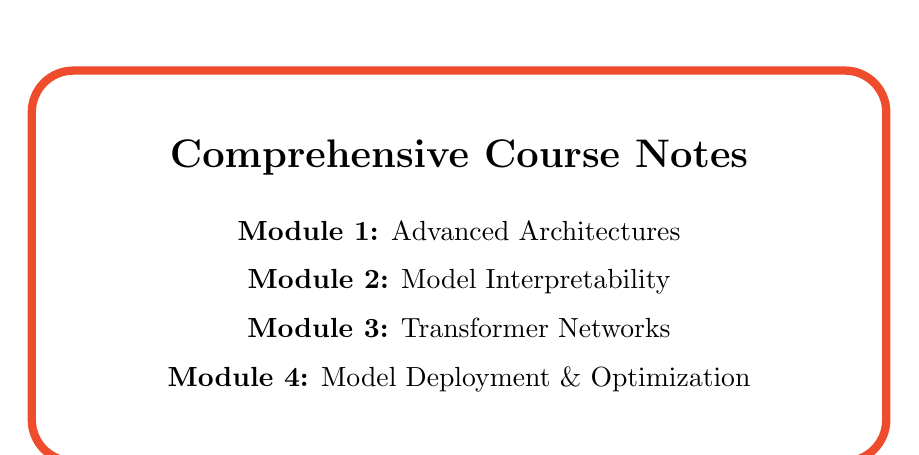
\begin{tikzpicture}
        \node[draw=pytorchcolor, line width=3pt, rounded corners=15pt, inner sep=25pt, fill=white] {
            \begin{minipage}{0.75\textwidth}
                \centering
                \Large\textbf{Comprehensive Course Notes}\\[0.5cm]
                \normalsize
                \textbf{Module 1:} Advanced Architectures\\[0.2cm]
                \textbf{Module 2:} Model Interpretability\\[0.2cm]
                \textbf{Module 3:} Transformer Networks\\[0.2cm]
                \textbf{Module 4:} Model Deployment \& Optimization
            \end{minipage}
        };
    \end{tikzpicture}
    
    \vfill
    
    \begin{tikzpicture}
        \draw[pytorchcolor, line width=2pt] (0,0) -- (12,0);
    \end{tikzpicture}
    
    \vspace{1cm}
    {\large PyTorch Deep Learning Specialization}\\[0.5cm]
    {\large\today}
\end{titlepage}

% Table of Contents
\tableofcontents
\newpage

%==============================================================================
% MODULE 1: ADVANCED ARCHITECTURES
%==============================================================================
\section{Module 1: Advanced Architectures}

\subsection{Inverted Residual Blocks}

\begin{conceptbox}[MobileNet Architecture]
MobileNets use \textbf{Inverted Residual Blocks} for efficiency:
\begin{itemize}
    \item \textbf{Standard Residual:} Wide $\to$ Narrow $\to$ Wide
    \item \textbf{Inverted Residual:} Narrow $\to$ Wide $\to$ Narrow
\end{itemize}
The "inverted" design expands channels in the middle for expressiveness, then compresses for efficiency.
\end{conceptbox}

\begin{lstlisting}[caption=Inverted Residual Block]
class InvertedResidualBlock(nn.Module):
    def __init__(self, in_channels, out_channels, 
                 expansion_factor=6, stride=1):
        super().__init__()
        
        hidden_dim = in_channels * expansion_factor
        self.use_residual = (stride == 1 and 
                            in_channels == out_channels)
        
        self.block = nn.Sequential(
            # 1x1 Expansion
            nn.Conv2d(in_channels, hidden_dim, 1, bias=False),
            nn.BatchNorm2d(hidden_dim),
            nn.ReLU6(inplace=True),
            
            # 3x3 Depthwise
            nn.Conv2d(hidden_dim, hidden_dim, 3, 
                     stride=stride, padding=1,
                     groups=hidden_dim, bias=False),
            nn.BatchNorm2d(hidden_dim),
            nn.ReLU6(inplace=True),
            
            # 1x1 Projection (no activation)
            nn.Conv2d(hidden_dim, out_channels, 1, bias=False),
            nn.BatchNorm2d(out_channels)
        )
    
    def forward(self, x):
        if self.use_residual:
            return x + self.block(x)  # Skip connection
        return self.block(x)
\end{lstlisting}

\begin{importantbox}[Depthwise Separable Convolution]
Standard convolution: $K \times K \times C_{in} \times C_{out}$ parameters

Depthwise Separable:
\begin{enumerate}
    \item \textbf{Depthwise:} $K \times K \times 1$ per channel (groups=C)
    \item \textbf{Pointwise:} $1 \times 1 \times C_{in} \times C_{out}$
\end{enumerate}
Reduces parameters by factor of $\approx K^2$
\end{importantbox}

\subsection{Siamese Networks}

\begin{conceptbox}[Siamese Architecture]
Twin networks that share weights, used for:
\begin{itemize}
    \item \textbf{One-shot learning:} Learn from few examples
    \item \textbf{Similarity matching:} Face verification, signature verification
    \item \textbf{Metric learning:} Learning embeddings where similar items are close
\end{itemize}
\end{conceptbox}

\begin{lstlisting}[caption=Siamese Network]
class SiameseNetwork(nn.Module):
    def __init__(self, embedding_dim=128):
        super().__init__()
        
        # Shared encoder
        self.encoder = nn.Sequential(
            nn.Conv2d(1, 32, 3, padding=1),
            nn.ReLU(),
            nn.MaxPool2d(2),
            nn.Conv2d(32, 64, 3, padding=1),
            nn.ReLU(),
            nn.MaxPool2d(2),
            nn.Flatten(),
            nn.Linear(64 * 7 * 7, embedding_dim)
        )
    
    def forward_one(self, x):
        return self.encoder(x)
    
    def forward(self, x1, x2):
        # Both inputs go through same encoder
        emb1 = self.forward_one(x1)
        emb2 = self.forward_one(x2)
        return emb1, emb2
\end{lstlisting}

\subsection{Triplet Loss}

\begin{formulabox}[Triplet Loss Function]
$$\mathcal{L} = \max(0, \|f(a) - f(p)\|^2 - \|f(a) - f(n)\|^2 + \alpha)$$

Where:
\begin{itemize}
    \item $a$ = anchor sample
    \item $p$ = positive (same class as anchor)
    \item $n$ = negative (different class)
    \item $\alpha$ = margin (typically 0.2 to 1.0)
\end{itemize}

\textbf{Goal:} Push negatives away, pull positives closer
\end{formulabox}

\begin{lstlisting}[caption=Triplet Loss Implementation]
class TripletLoss(nn.Module):
    def __init__(self, margin=1.0):
        super().__init__()
        self.margin = margin
    
    def forward(self, anchor, positive, negative):
        pos_dist = F.pairwise_distance(anchor, positive)
        neg_dist = F.pairwise_distance(anchor, negative)
        
        loss = F.relu(pos_dist - neg_dist + self.margin)
        return loss.mean()

# Usage
model = SiameseNetwork()
criterion = TripletLoss(margin=1.0)

anchor_emb = model.forward_one(anchor_img)
pos_emb = model.forward_one(positive_img)
neg_emb = model.forward_one(negative_img)

loss = criterion(anchor_emb, pos_emb, neg_emb)
\end{lstlisting}

\begin{tipbox}[Triplet Mining Strategies]
\begin{itemize}
    \item \textbf{Random:} Random triplet selection (easy, less effective)
    \item \textbf{Hard:} Hardest positive and negative per anchor
    \item \textbf{Semi-Hard:} Negatives farther than positive but within margin
\end{itemize}
\end{tipbox}

\subsection{Contrastive Loss}

\begin{formulabox}[Contrastive Loss]
For pairs of samples:
$$\mathcal{L} = (1-y) \cdot D^2 + y \cdot \max(0, m - D)^2$$

Where:
\begin{itemize}
    \item $y=0$ for similar pairs, $y=1$ for dissimilar
    \item $D$ = distance between embeddings
    \item $m$ = margin
\end{itemize}
\end{formulabox}

\newpage
%==============================================================================
% MODULE 2: MODEL INTERPRETABILITY
%==============================================================================
\section{Module 2: Model Interpretability}

\subsection{Why Interpretability Matters}

\begin{conceptbox}[Interpretability Goals]
\begin{itemize}
    \item \textbf{Debugging:} Understanding model failures
    \item \textbf{Trust:} Building confidence in predictions
    \item \textbf{Compliance:} Meeting regulatory requirements
    \item \textbf{Improvement:} Identifying what features matter
\end{itemize}
\end{conceptbox}

\subsection{Forward Hooks}

\begin{importantbox}[Hook Mechanism]
Hooks allow intercepting data during forward/backward pass without modifying the model.
\end{importantbox}

\begin{lstlisting}[caption=Registering Forward Hooks]
# Storage for activations
activations = {}

def get_activation(name):
    def hook(model, input, output):
        activations[name] = output.detach()
    return hook

# Register hook on a layer
model.features[7].register_forward_hook(get_activation('conv7'))

# Forward pass
output = model(input_image)

# Access stored activations
conv7_features = activations['conv7']
print(conv7_features.shape)  # [batch, channels, H, W]
\end{lstlisting}

\subsection{Saliency Maps}

\begin{conceptbox}[Saliency (Gradient-based)]
Shows which input pixels most affect the output by computing gradients of the output with respect to input pixels.
\end{conceptbox}

\begin{lstlisting}[caption=Computing Saliency Maps]
def compute_saliency(model, image, target_class):
    model.eval()
    image.requires_grad_()
    
    # Forward pass
    output = model(image)
    
    # Backward pass for target class
    output[0, target_class].backward()
    
    # Get gradients
    saliency = image.grad.abs()
    
    # Take max across channels
    saliency = saliency.max(dim=1)[0]  # [B, H, W]
    
    return saliency

# Usage
saliency_map = compute_saliency(model, image, predicted_class)

# Visualize
plt.imshow(saliency_map.squeeze().cpu(), cmap='hot')
plt.title('Saliency Map')
\end{lstlisting}

\subsection{Class Activation Maps (CAM)}

\begin{conceptbox}[CAM Intuition]
CAM shows which regions of an image are important for a specific class prediction. Uses Global Average Pooling (GAP) layer weights.
\end{conceptbox}

\begin{formulabox}[CAM Formula]
$$M_c(x,y) = \sum_k w_k^c \cdot A_k(x,y)$$

Where:
\begin{itemize}
    \item $A_k$ = activation map from last conv layer
    \item $w_k^c$ = weight connecting feature $k$ to class $c$
\end{itemize}
\end{formulabox}

\begin{lstlisting}[caption=Computing CAM]
def compute_cam(model, image, target_class):
    model.eval()
    features = None
    
    # Hook to capture last conv output
    def hook_fn(module, input, output):
        nonlocal features
        features = output.detach()
    
    # Register hook (adjust layer name for your model)
    hook = model.features[-1].register_forward_hook(hook_fn)
    
    # Forward pass
    output = model(image)
    hook.remove()
    
    # Get classifier weights
    weights = model.classifier[-1].weight[target_class]
    
    # Compute weighted sum of feature maps
    cam = torch.zeros(features.shape[2:])
    for i, w in enumerate(weights):
        cam += w * features[0, i, :, :]
    
    # Normalize
    cam = F.relu(cam)  # Keep positive
    cam = cam - cam.min()
    cam = cam / cam.max()
    
    # Resize to input size
    cam = F.interpolate(
        cam.unsqueeze(0).unsqueeze(0),
        size=image.shape[2:],
        mode='bilinear'
    ).squeeze()
    
    return cam
\end{lstlisting}

\subsection{Grad-CAM}

\begin{conceptbox}[Grad-CAM]
Generalization of CAM that works with any CNN architecture (not just those with GAP). Uses gradients instead of classifier weights.
\end{conceptbox}

\begin{lstlisting}[caption=Grad-CAM Implementation]
def grad_cam(model, image, target_class, target_layer):
    model.eval()
    gradients = None
    activations = None
    
    def forward_hook(module, input, output):
        nonlocal activations
        activations = output.detach()
    
    def backward_hook(module, grad_in, grad_out):
        nonlocal gradients
        gradients = grad_out[0].detach()
    
    # Register hooks
    fwd_hook = target_layer.register_forward_hook(forward_hook)
    bwd_hook = target_layer.register_full_backward_hook(backward_hook)
    
    # Forward + backward
    output = model(image)
    model.zero_grad()
    output[0, target_class].backward()
    
    # Remove hooks
    fwd_hook.remove()
    bwd_hook.remove()
    
    # Compute importance weights (global average of gradients)
    weights = gradients.mean(dim=[2, 3], keepdim=True)
    
    # Weighted combination
    grad_cam = F.relu((weights * activations).sum(dim=1, keepdim=True))
    
    # Normalize and resize
    grad_cam = F.interpolate(grad_cam, size=image.shape[2:], mode='bilinear')
    grad_cam = (grad_cam - grad_cam.min()) / (grad_cam.max() - grad_cam.min())
    
    return grad_cam.squeeze()
\end{lstlisting}

\subsection{Visualizing Feature Maps}

\begin{lstlisting}[caption=Feature Map Visualization]
def visualize_feature_maps(feature_maps, num_cols=8):
    """Visualize feature maps from a conv layer"""
    n_features = feature_maps.shape[1]
    num_rows = (n_features + num_cols - 1) // num_cols
    
    fig, axes = plt.subplots(num_rows, num_cols, 
                              figsize=(num_cols*2, num_rows*2))
    
    for i, ax in enumerate(axes.flat):
        if i < n_features:
            ax.imshow(feature_maps[0, i].cpu(), cmap='viridis')
        ax.axis('off')
    
    plt.tight_layout()
    plt.show()
\end{lstlisting}

\newpage
%==============================================================================
% MODULE 3: TRANSFORMER NETWORKS
%==============================================================================
\section{Module 3: Transformer Networks}

\subsection{Transformer Architecture Overview}

\begin{conceptbox}[Key Components]
\begin{enumerate}
    \item \textbf{Multi-Head Self-Attention:} Learn relationships between positions
    \item \textbf{Positional Encoding:} Inject sequence order information
    \item \textbf{Feed-Forward Network:} Per-position transformations
    \item \textbf{Layer Normalization:} Stabilize training
    \item \textbf{Residual Connections:} Enable gradient flow
\end{enumerate}
\end{conceptbox}

\subsection{Self-Attention Mechanism}

\begin{formulabox}[Scaled Dot-Product Attention]
$$\text{Attention}(Q, K, V) = \text{softmax}\left(\frac{QK^T}{\sqrt{d_k}}\right)V$$

Where:
\begin{itemize}
    \item $Q$ = Query matrix (what we're looking for)
    \item $K$ = Key matrix (what we're comparing against)
    \item $V$ = Value matrix (what we extract)
    \item $d_k$ = Key dimension (scaling factor)
\end{itemize}
\end{formulabox}

\begin{lstlisting}[caption=Self-Attention Implementation]
class SelfAttention(nn.Module):
    def __init__(self, embed_dim, num_heads):
        super().__init__()
        self.embed_dim = embed_dim
        self.num_heads = num_heads
        self.head_dim = embed_dim // num_heads
        
        self.qkv = nn.Linear(embed_dim, 3 * embed_dim)
        self.proj = nn.Linear(embed_dim, embed_dim)
        self.scale = self.head_dim ** -0.5
    
    def forward(self, x, mask=None):
        B, T, C = x.shape
        
        # Compute Q, K, V
        qkv = self.qkv(x).reshape(B, T, 3, self.num_heads, self.head_dim)
        qkv = qkv.permute(2, 0, 3, 1, 4)  # [3, B, heads, T, head_dim]
        q, k, v = qkv[0], qkv[1], qkv[2]
        
        # Attention scores
        attn = (q @ k.transpose(-2, -1)) * self.scale
        
        if mask is not None:
            attn = attn.masked_fill(mask == 0, float('-inf'))
        
        attn = attn.softmax(dim=-1)
        
        # Apply attention to values
        out = (attn @ v).transpose(1, 2).reshape(B, T, C)
        return self.proj(out)
\end{lstlisting}

\subsection{Multi-Head Attention}

\begin{importantbox}[Why Multiple Heads?]
Each head can learn different types of relationships:
\begin{itemize}
    \item One head might focus on syntax
    \item Another on semantics
    \item Another on long-range dependencies
\end{itemize}
Typical: 8-16 heads in transformers
\end{importantbox}

\subsection{Positional Encoding}

\begin{lstlisting}[caption=Sinusoidal Positional Encoding]
class PositionalEncoding(nn.Module):
    def __init__(self, d_model, max_len=5000, dropout=0.1):
        super().__init__()
        self.dropout = nn.Dropout(dropout)
        
        pe = torch.zeros(max_len, d_model)
        position = torch.arange(max_len).unsqueeze(1).float()
        
        div_term = torch.exp(
            torch.arange(0, d_model, 2).float() * 
            (-math.log(10000.0) / d_model)
        )
        
        pe[:, 0::2] = torch.sin(position * div_term)  # Even
        pe[:, 1::2] = torch.cos(position * div_term)  # Odd
        
        self.register_buffer('pe', pe.unsqueeze(0))
    
    def forward(self, x):
        x = x + self.pe[:, :x.size(1)]
        return self.dropout(x)
\end{lstlisting}

\subsection{Transformer Encoder Block}

\begin{lstlisting}[caption=Encoder Block]
class TransformerEncoderBlock(nn.Module):
    def __init__(self, embed_dim, num_heads, ff_dim, dropout=0.1):
        super().__init__()
        
        self.attention = nn.MultiheadAttention(
            embed_dim, num_heads, dropout=dropout, batch_first=True
        )
        
        self.ffn = nn.Sequential(
            nn.Linear(embed_dim, ff_dim),
            nn.GELU(),
            nn.Dropout(dropout),
            nn.Linear(ff_dim, embed_dim),
            nn.Dropout(dropout)
        )
        
        self.norm1 = nn.LayerNorm(embed_dim)
        self.norm2 = nn.LayerNorm(embed_dim)
        self.dropout = nn.Dropout(dropout)
    
    def forward(self, x, mask=None):
        # Self-attention with residual
        attn_out, _ = self.attention(x, x, x, attn_mask=mask)
        x = self.norm1(x + self.dropout(attn_out))
        
        # FFN with residual
        ffn_out = self.ffn(x)
        x = self.norm2(x + ffn_out)
        
        return x
\end{lstlisting}

\subsection{Transformer Decoder}

\begin{lstlisting}[caption=Decoder Block with Causal Mask]
class TransformerDecoderBlock(nn.Module):
    def __init__(self, embed_dim, num_heads, ff_dim, dropout=0.1):
        super().__init__()
        
        # Masked self-attention
        self.self_attn = nn.MultiheadAttention(
            embed_dim, num_heads, dropout=dropout, batch_first=True
        )
        
        # Cross-attention
        self.cross_attn = nn.MultiheadAttention(
            embed_dim, num_heads, dropout=dropout, batch_first=True
        )
        
        self.ffn = nn.Sequential(
            nn.Linear(embed_dim, ff_dim),
            nn.GELU(),
            nn.Linear(ff_dim, embed_dim)
        )
        
        self.norm1 = nn.LayerNorm(embed_dim)
        self.norm2 = nn.LayerNorm(embed_dim)
        self.norm3 = nn.LayerNorm(embed_dim)
    
    def forward(self, x, encoder_output, tgt_mask=None):
        # Masked self-attention
        attn1, _ = self.self_attn(x, x, x, attn_mask=tgt_mask)
        x = self.norm1(x + attn1)
        
        # Cross-attention with encoder output
        attn2, _ = self.cross_attn(x, encoder_output, encoder_output)
        x = self.norm2(x + attn2)
        
        # FFN
        x = self.norm3(x + self.ffn(x))
        return x

# Causal mask (prevent seeing future tokens)
def generate_causal_mask(size):
    mask = torch.triu(torch.ones(size, size), diagonal=1).bool()
    return mask
\end{lstlisting}

\subsection{Complete Seq2Seq Transformer}

\begin{lstlisting}[caption=Translation Transformer]
class Transformer(nn.Module):
    def __init__(self, src_vocab, tgt_vocab, d_model=512, 
                 n_heads=8, n_layers=6, ff_dim=2048):
        super().__init__()
        
        self.src_embed = nn.Embedding(src_vocab, d_model)
        self.tgt_embed = nn.Embedding(tgt_vocab, d_model)
        self.pos_enc = PositionalEncoding(d_model)
        
        self.encoder = nn.TransformerEncoder(
            nn.TransformerEncoderLayer(d_model, n_heads, ff_dim),
            num_layers=n_layers
        )
        
        self.decoder = nn.TransformerDecoder(
            nn.TransformerDecoderLayer(d_model, n_heads, ff_dim),
            num_layers=n_layers
        )
        
        self.output = nn.Linear(d_model, tgt_vocab)
    
    def forward(self, src, tgt, tgt_mask=None):
        # Encode source
        src_emb = self.pos_enc(self.src_embed(src))
        memory = self.encoder(src_emb)
        
        # Decode target
        tgt_emb = self.pos_enc(self.tgt_embed(tgt))
        out = self.decoder(tgt_emb, memory, tgt_mask=tgt_mask)
        
        return self.output(out)
\end{lstlisting}

\newpage
%==============================================================================
% MODULE 4: MODEL DEPLOYMENT & OPTIMIZATION
%==============================================================================
\section{Module 4: Model Deployment \& Optimization}

\subsection{Experiment Tracking with MLflow}

\begin{lstlisting}[caption=MLflow Integration]
import mlflow
import mlflow.pytorch

# Start experiment
mlflow.set_experiment("my_experiment")

with mlflow.start_run():
    # Log parameters
    mlflow.log_param("learning_rate", 0.001)
    mlflow.log_param("batch_size", 32)
    mlflow.log_param("epochs", 10)
    
    # Training loop
    for epoch in range(epochs):
        train_loss = train_epoch(...)
        val_acc = validate(...)
        
        # Log metrics
        mlflow.log_metric("train_loss", train_loss, step=epoch)
        mlflow.log_metric("val_accuracy", val_acc, step=epoch)
    
    # Log model
    mlflow.pytorch.log_model(model, "model")
    
    # Log artifacts (files)
    mlflow.log_artifact("config.yaml")
\end{lstlisting}

\subsection{ONNX Export}

\begin{conceptbox}[Why ONNX?]
Open Neural Network Exchange (ONNX) enables:
\begin{itemize}
    \item Cross-framework compatibility
    \item Optimized inference runtimes
    \item Edge deployment (mobile, IoT)
    \item Production serving
\end{itemize}
\end{conceptbox}

\begin{lstlisting}[caption=Exporting to ONNX]
import torch.onnx

# Set model to evaluation mode
model.eval()

# Create dummy input matching expected shape
dummy_input = torch.randn(1, 3, 224, 224)

# Export
torch.onnx.export(
    model,
    dummy_input,
    "model.onnx",
    input_names=['input'],
    output_names=['output'],
    dynamic_axes={
        'input': {0: 'batch_size'},
        'output': {0: 'batch_size'}
    },
    opset_version=11
)

# Verify export
import onnx
onnx_model = onnx.load("model.onnx")
onnx.checker.check_model(onnx_model)
\end{lstlisting}

\begin{lstlisting}[caption=ONNX Runtime Inference]
import onnxruntime as ort

# Load model
session = ort.InferenceSession("model.onnx")

# Prepare input
input_data = preprocess(image).numpy()

# Run inference
outputs = session.run(
    None,  # Output names (None = all)
    {'input': input_data}
)

predictions = outputs[0]
\end{lstlisting}

\subsection{Model Pruning}

\begin{conceptbox}[Pruning Types]
\begin{itemize}
    \item \textbf{Unstructured:} Remove individual weights (sparse tensors)
    \item \textbf{Structured:} Remove entire channels/filters (faster inference)
\end{itemize}
\end{conceptbox}

\begin{lstlisting}[caption=Pruning Implementation]
import torch.nn.utils.prune as prune

# Unstructured pruning (L1 norm based)
prune.l1_unstructured(
    model.conv1, 
    name='weight', 
    amount=0.3  # Prune 30% of weights
)

# Structured pruning (remove channels)
prune.ln_structured(
    model.conv1,
    name='weight',
    amount=0.2,     # Remove 20% of channels
    n=2,            # L2 norm
    dim=0           # Prune along output channels
)

# Check sparsity
total = 0
zero = 0
for name, module in model.named_modules():
    if hasattr(module, 'weight'):
        total += module.weight.numel()
        zero += (module.weight == 0).sum().item()
print(f"Sparsity: {100 * zero / total:.1f}%")

# Make pruning permanent
prune.remove(model.conv1, 'weight')
\end{lstlisting}

\begin{tipbox}[Iterative Pruning]
Best results come from iterative pruning:
\begin{enumerate}
    \item Train full model
    \item Prune small percentage
    \item Fine-tune
    \item Repeat
\end{enumerate}
\end{tipbox}

\subsection{Model Quantization}

\begin{importantbox}[Quantization Benefits]
\begin{itemize}
    \item Reduces model size (FP32 $\to$ INT8 = 4× smaller)
    \item Faster inference on CPU
    \item Lower memory bandwidth
    \item Better for edge devices
\end{itemize}
\end{importantbox}

\subsubsection{Dynamic Quantization}

\begin{lstlisting}[caption=Dynamic Quantization]
import torch.quantization

# Quantize Linear and LSTM layers
quantized_model = torch.quantization.quantize_dynamic(
    model,
    {nn.Linear, nn.LSTM},  # Layers to quantize
    dtype=torch.qint8
)

# Compare sizes
def model_size(model):
    torch.save(model.state_dict(), "temp.pt")
    size = os.path.getsize("temp.pt") / 1e6
    os.remove("temp.pt")
    return size

print(f"Original: {model_size(model):.2f} MB")
print(f"Quantized: {model_size(quantized_model):.2f} MB")
\end{lstlisting}

\subsubsection{Static Quantization}

\begin{lstlisting}[caption=Static Quantization]
# Prepare model
model.eval()
model.qconfig = torch.quantization.get_default_qconfig('fbgemm')
model_prepared = torch.quantization.prepare(model)

# Calibrate with representative data
with torch.no_grad():
    for inputs, _ in calibration_loader:
        model_prepared(inputs)

# Convert to quantized
quantized_model = torch.quantization.convert(model_prepared)
\end{lstlisting}

\subsubsection{Quantization-Aware Training (QAT)}

\begin{lstlisting}[caption=QAT Pipeline]
# Prepare model for QAT
model.train()
model.qconfig = torch.quantization.get_default_qat_qconfig('fbgemm')
model_prepared = torch.quantization.prepare_qat(model)

# Train with fake quantization
for epoch in range(num_epochs):
    for inputs, targets in train_loader:
        outputs = model_prepared(inputs)
        loss = criterion(outputs, targets)
        loss.backward()
        optimizer.step()

# Convert to fully quantized
model_prepared.eval()
quantized_model = torch.quantization.convert(model_prepared)
\end{lstlisting}

\subsection{Model Optimization Comparison}

\begin{center}
\begin{tabular}{lccc}
\toprule
\textbf{Technique} & \textbf{Size $\downarrow$} & \textbf{Speed $\uparrow$} & \textbf{Accuracy} \\
\midrule
Pruning (30\%) & 30\% & Moderate & Slight drop \\
Dynamic Quant & 75\% & 2-4× & Minimal drop \\
Static Quant & 75\% & 2-4× & Minimal drop \\
QAT & 75\% & 2-4× & Best preserved \\
ONNX Runtime & 0\% & 1.5-2× & None \\
\bottomrule
\end{tabular}
\end{center}

\subsection{TorchScript}

\begin{lstlisting}[caption=TorchScript Export]
# Tracing (for models without control flow)
traced = torch.jit.trace(model, example_input)
traced.save("model_traced.pt")

# Scripting (preserves control flow)
scripted = torch.jit.script(model)
scripted.save("model_scripted.pt")

# Load and use
loaded = torch.jit.load("model_traced.pt")
output = loaded(input_tensor)
\end{lstlisting}

\newpage
%==============================================================================
% QUIZ REVIEW
%==============================================================================
\section{Quiz Review: Key Concepts}

\subsection{Quiz 9: Advanced Architectures}

\begin{enumerate}
    \item \textbf{Inverted Residual:} Expand $\to$ Depthwise $\to$ Project
    \item \textbf{Depthwise conv:} groups=in\_channels (one filter per channel)
    \item ReLU6 clips values at 6 (stable for fixed-point)
    \item \textbf{Siamese:} Two networks, shared weights
    \item \textbf{Triplet loss:} anchor, positive, negative
    \item Margin ensures negative is farther than positive
    \item Embedding similarity: cosine or Euclidean distance
    \item One-shot learning from few examples
    \item Skip connection when stride=1 AND in\_channels=out\_channels
    \item Expansion factor controls width of hidden layer
\end{enumerate}

\subsection{Quiz 10: Model Interpretability}

\begin{enumerate}
    \item \textbf{Forward hooks:} Capture activations during inference
    \item Hooks receive (model, input, output)
    \item \textbf{Saliency:} Gradient of output w.r.t. input
    \item \textbf{CAM:} Weighted sum of last conv features
    \item Grad-CAM works with any architecture
    \item \texttt{register\_forward\_hook()} for forward pass
    \item Remove hooks when done to avoid memory leaks
    \item Feature visualization shows what neurons detect
    \item Interpretability helps debugging and trust
    \item \texttt{output.backward()} for gradient computation
\end{enumerate}

\subsection{Quiz 11: Transformers}

\begin{enumerate}
    \item \textbf{Self-attention:} Relates all positions to each other
    \item Scaling by $\sqrt{d_k}$ prevents vanishing gradients
    \item \textbf{Multi-head:} Multiple attention patterns in parallel
    \item \textbf{Positional encoding:} Injects sequence order
    \item Encoder: bidirectional, Decoder: causal (masked)
    \item \textbf{Cross-attention:} Decoder attends to encoder output
    \item LayerNorm applied after each sub-layer
    \item FFN: two linear layers with activation
    \item \texttt{nn.MultiheadAttention} in PyTorch
    \item Causal mask: upper triangular ones
\end{enumerate}

\subsection{Quiz 12: Deployment}

\begin{enumerate}
    \item \textbf{ONNX:} Cross-platform model format
    \item \textbf{MLflow:} Experiment tracking and model registry
    \item \textbf{Pruning:} Remove unimportant weights
    \item \textbf{Dynamic quantization:} Quantize at runtime
    \item \textbf{Static quantization:} Pre-computed quantization params
    \item \textbf{QAT:} Train with fake quantization
    \item INT8 = 4× smaller than FP32
    \item \texttt{torch.onnx.export()} for conversion
    \item dynamic\_axes for variable batch size
    \item Calibration data needed for static quantization
\end{enumerate}

\newpage
%==============================================================================
% QUICK REFERENCE
%==============================================================================
\section{Quick Reference}

\subsection{Siamese Network Template}

\begin{lstlisting}
class SiameseNet(nn.Module):
    def __init__(self):
        super().__init__()
        self.encoder = nn.Sequential(...)  # Shared
    
    def forward(self, x1, x2):
        return self.encoder(x1), self.encoder(x2)

# Triplet loss
loss = F.relu(pos_dist - neg_dist + margin).mean()
\end{lstlisting}

\subsection{Hook Template}

\begin{lstlisting}
activations = {}

def hook(model, input, output):
    activations['layer'] = output.detach()

handle = model.layer.register_forward_hook(hook)
output = model(x)  # Activations captured
handle.remove()    # Clean up
\end{lstlisting}

\subsection{ONNX Export Template}

\begin{lstlisting}
model.eval()
dummy = torch.randn(1, 3, 224, 224)
torch.onnx.export(model, dummy, "model.onnx",
                  input_names=['input'],
                  output_names=['output'],
                  dynamic_axes={'input': {0: 'batch'},
                               'output': {0: 'batch'}})
\end{lstlisting}

\subsection{Quantization Template}

\begin{lstlisting}
# Dynamic (easiest)
model_q = torch.quantization.quantize_dynamic(
    model, {nn.Linear}, dtype=torch.qint8)

# Static
model.qconfig = torch.quantization.get_default_qconfig('fbgemm')
model_prep = torch.quantization.prepare(model)
# Calibrate...
model_q = torch.quantization.convert(model_prep)
\end{lstlisting}

\subsection{Transformer Template}

\begin{lstlisting}
encoder_layer = nn.TransformerEncoderLayer(
    d_model=512, nhead=8, dim_feedforward=2048)
encoder = nn.TransformerEncoder(encoder_layer, num_layers=6)

decoder_layer = nn.TransformerDecoderLayer(
    d_model=512, nhead=8, dim_feedforward=2048)
decoder = nn.TransformerDecoder(decoder_layer, num_layers=6)
\end{lstlisting}

\end{document}
